% !TEX root = ../thesis.tex
\section{Example Interactive Visualizations}
\label{sec:vl:examples}

Vega-Lite's design is motivated by two goals: to enable rapid yet expressive
specification of interactive visualizations, and to do so with concise
primitives that facilitate systematic enumeration and exploration of design
variations. In this section, we demonstrate how these goals are addressed using
a range of example interactive visualizations. To evaluate expressivity, we once
again choose examples that cover Yi et al.'s~\cite{yi:understanding} taxonomy of
interaction methods. Recall, the taxonomy identifies seven categories of
techniques: \emph{select}, to mark items of interest; \emph{explore} to examine
subsets of the data; \emph{connect} to highlight related items within and across
views; \emph{abstract/elaborate} to vary the level of detail; \emph{reconfigure}
to show different arrangements of the data; \emph{filter} to show elements
conditionally; and, \emph{encode}, to change the visual representations used. To
assess authoring speed, we compare our specifications against canonical Reactive
Vega examples~\cite{reactive-vega-arch, reactive-vega-model, vega:editor}. Where
applicable, we also show how construction of our examples can be systematically
varied to explore alternate points in the design space.

\subsection{Selection: Click/Shift-Click and Brushing}

\cref{fig:vl:singleSelection} provides the full Vega-Lite specification for a
scatterplot where users can mark individual points of interest. It includes the
simplest definition of a selection\,---\,a name and type\,---\,and illustrates
how the mark color is determined conditionally.

Modifying a single property, \emph{type}, as in \cref{fig:vl:multiSelection},
allows users to mark multiple points (\emph{toggle} is automatically
instantiated by the compiler, but we explicitly specify it in the figure for
clarity). We can instead add \emph{project} (\cref{fig:vl:projectSingle})
such that marking a single point of interest highlights all other points that
share particular data values\,---\,a \emph{connect}-type interaction. Such
changes to the specification are not mutually exclusive, and can be composed as
shown in \cref{fig:vl:projectMulti}.

By using the \emph{interval} type, users can mark items of interest within a
continuous region. As shown in \cref{fig:vl:intervalSelection}, the compiler
automatically adds a rectangle mark to depict the selection, and instantiates
\emph{translate} to allow it to be repositioned (\cref{fig:vl:translate}). In this
context, \emph{project} restricts the interval to a single dimension
(\cref{fig:vl:projectInterval}).

These specifications are an order of magnitude more concise than their Vega
counterparts. With Vega-Lite, users need only specify the semantics of their
interaction and the compiler fills in appropriate default values. For example,
by default, individual points are selected on click and multiple points on
shift-click. Users can override these defaults, sometimes producing a
qualitatively different user experience. For example, one can instead update
selections on \texttt{mouseover} to produce a ``paint brush'' interaction, as in
\cref{fig:vl:paintbrush}. In contrast, with Vega, users need to manually author all
the components of an interaction technique, including determining whether event
properties need to be passed through scale inversions, creating necessary
backing data structures, and adding marks to represent a brush component.

\subsection{Explore \& Encode: Panning \& Zooming}
\label{sec:vl:panzoom}

Vega-Lite's selections also enable accretive design of interactions. Consider
our previous example of brushing a scatterplot. We can define an additional
interval selection and \emph{bind} it to the unit's scale functions
(\cref{fig:vl:bindScales}). The compiler populates the selection with the x and y
scale domains, parameterizes them to use it, and instantiates the
\emph{translate} and \emph{zoom} transforms. Users can now brush, pan, and zoom
the scatterplot. However, the default definitions of the two interval selections
collide: dragging produces a brush and pans the plot. This example illustrates
that concise methods for overriding defaults can not only be useful (as in
\cref{fig:vl:paintbrush}) but also necessary. We override the default events that
trigger the two interactions using Vega's event selector
syntax~\cite{reactive-vega-model}. As \cref{fig:vl:bindScales} shows, we specify
that brushing only occurs when the user drags with the shift key pressed.

The Vega-Lite specification for panning and zooming is, once again, more
succinct than the corresponding Vega example. However, it is more interesting to
compare the latter against the output specification produced by the Vega-Lite
compiler. The Vega example requires users to manually specify their initial
scale extents when defining the interaction. On the other hand, to enable
data-driven initialization of interval selections, the Vega-Lite output
calculates scale extents as part of a derived dataset in the output
specification, with additional transformations to offset these calculations for
the interaction. Such a construction is not idiomatic Vega, and would be
unintuitive for users to construct manually. Thus, Vega-Lite's higher-level
approach not only offers more rapid specification, but it can also enable
interactions that a user may not realize are expressible with lower-level
representations.

Moreover, by enabling this interaction through composable primitives (rather
than a single, specific ``pan and zoom'' operator~\cite{bostock:d3}), Vega-Lite
also facilitates exploring related interactions in the design space. For
example, using the \emph{project} transform, we can author a separate selection
for the x and y scales each, and selectively enable the \emph{translate} and
\emph{zoom} transforms. While such a combination may not be
desirable\,---\,panning only one scale while zooming the other\,---\,Vega-Lite's
selections nevertheless allow us to systematically identify it as a possible
design. Similarly, we could project over the color or size channels, thereby
allowing users to interactively vary the mappings specified by these scales. For
example, ``panning'' a heatmap's color legend to shift the high and low
intensity data values. If the selections were defined over the visual
\emph{range}, users could instead shift the colors used in a sequential color
scale.

\subsection{Connect: Brushing \& Linking}

We can wrap our previous example, from \cref{fig:vl:bindScales}, in a \emph{repeat}
operator to construct a scatterplot matrix (SPLOM) as shown in
\cref{fig:vl:resolveGlobal}. With no further modifications, all our previous
interactions now work within each cell of the SPLOM and are synchronized across
the others. For example, dragging pans not only the particular cell the user is
in, but related cells along shared axes. Similarly, dragging with the shift key
pressed produces a brush in the current cell, and highlights points across all
cells that fall within it.

As its name suggests, the repeat operator creates one instance of the child
specification for the given parameters. By default, to provide a consistent
experience when moving from a unit to a composite specification, Vega-Lite
creates a \emph{global} instance of the selection that is populated and shared
between all repeated instances (\cref{fig:vl:resolveGlobal}). With the
\emph{resolve} property, users can specify alternate disambiguation methods
including creating an independent brush for each cell, unioning the brushes, or
intersecting them
(\cref{fig:vl:resolveIndependent,fig:vl:resolveUnion,fig:vl:resolveIntersect}
respectively). If selections are bound to scales or parameterize them, only a
global selection is supported for consistency with the composition algebra.

With this example, it is more instructive to compare the amount of effort
required, with Vega-Lite and Vega, to move from a single interactive scatterplot
to an interactive SPLOM. While the Vega specifications for the two are broadly
similar, the latter requires an extra level of indirection to identify the
specific cell a user is interacting in, and to ensure that the correct data
values are used to determine inclusion within the brush. In Vega-Lite, this
complexity is succinctly encapsulated by the \emph{resolve} keyword which, as
discussed, can be systematically varied to explore alternatives. Mimicing
Vega-Lite's \emph{union} and \emph{intersect} behaviors is not trivial, and
requires unidiomatic Vega once more. Users cannot simply duplicate the
interaction logic for each cell manually, as the dimensions of the SPLOM are
determined by data.

\subsection{Abstract/Elaborate: Overview\,+\,Detail}

Thus far, selections have parameterized scale extents through the \emph{bind}
transform and previous examples have demonstrated how visualized data can be
abstracted/elaborated via zooming. The figure below shows how a selection
defined in one unit specification can be explicitly given as the scale domain of
another in a concatenated display. Doing so creates an overview\,+\,detail
interaction: brushing in the bottom (overview) chart displays only selected
items at a higher resolution in the larger (detail) chart at the top.

\begin{figure}[h!]
  \centering
  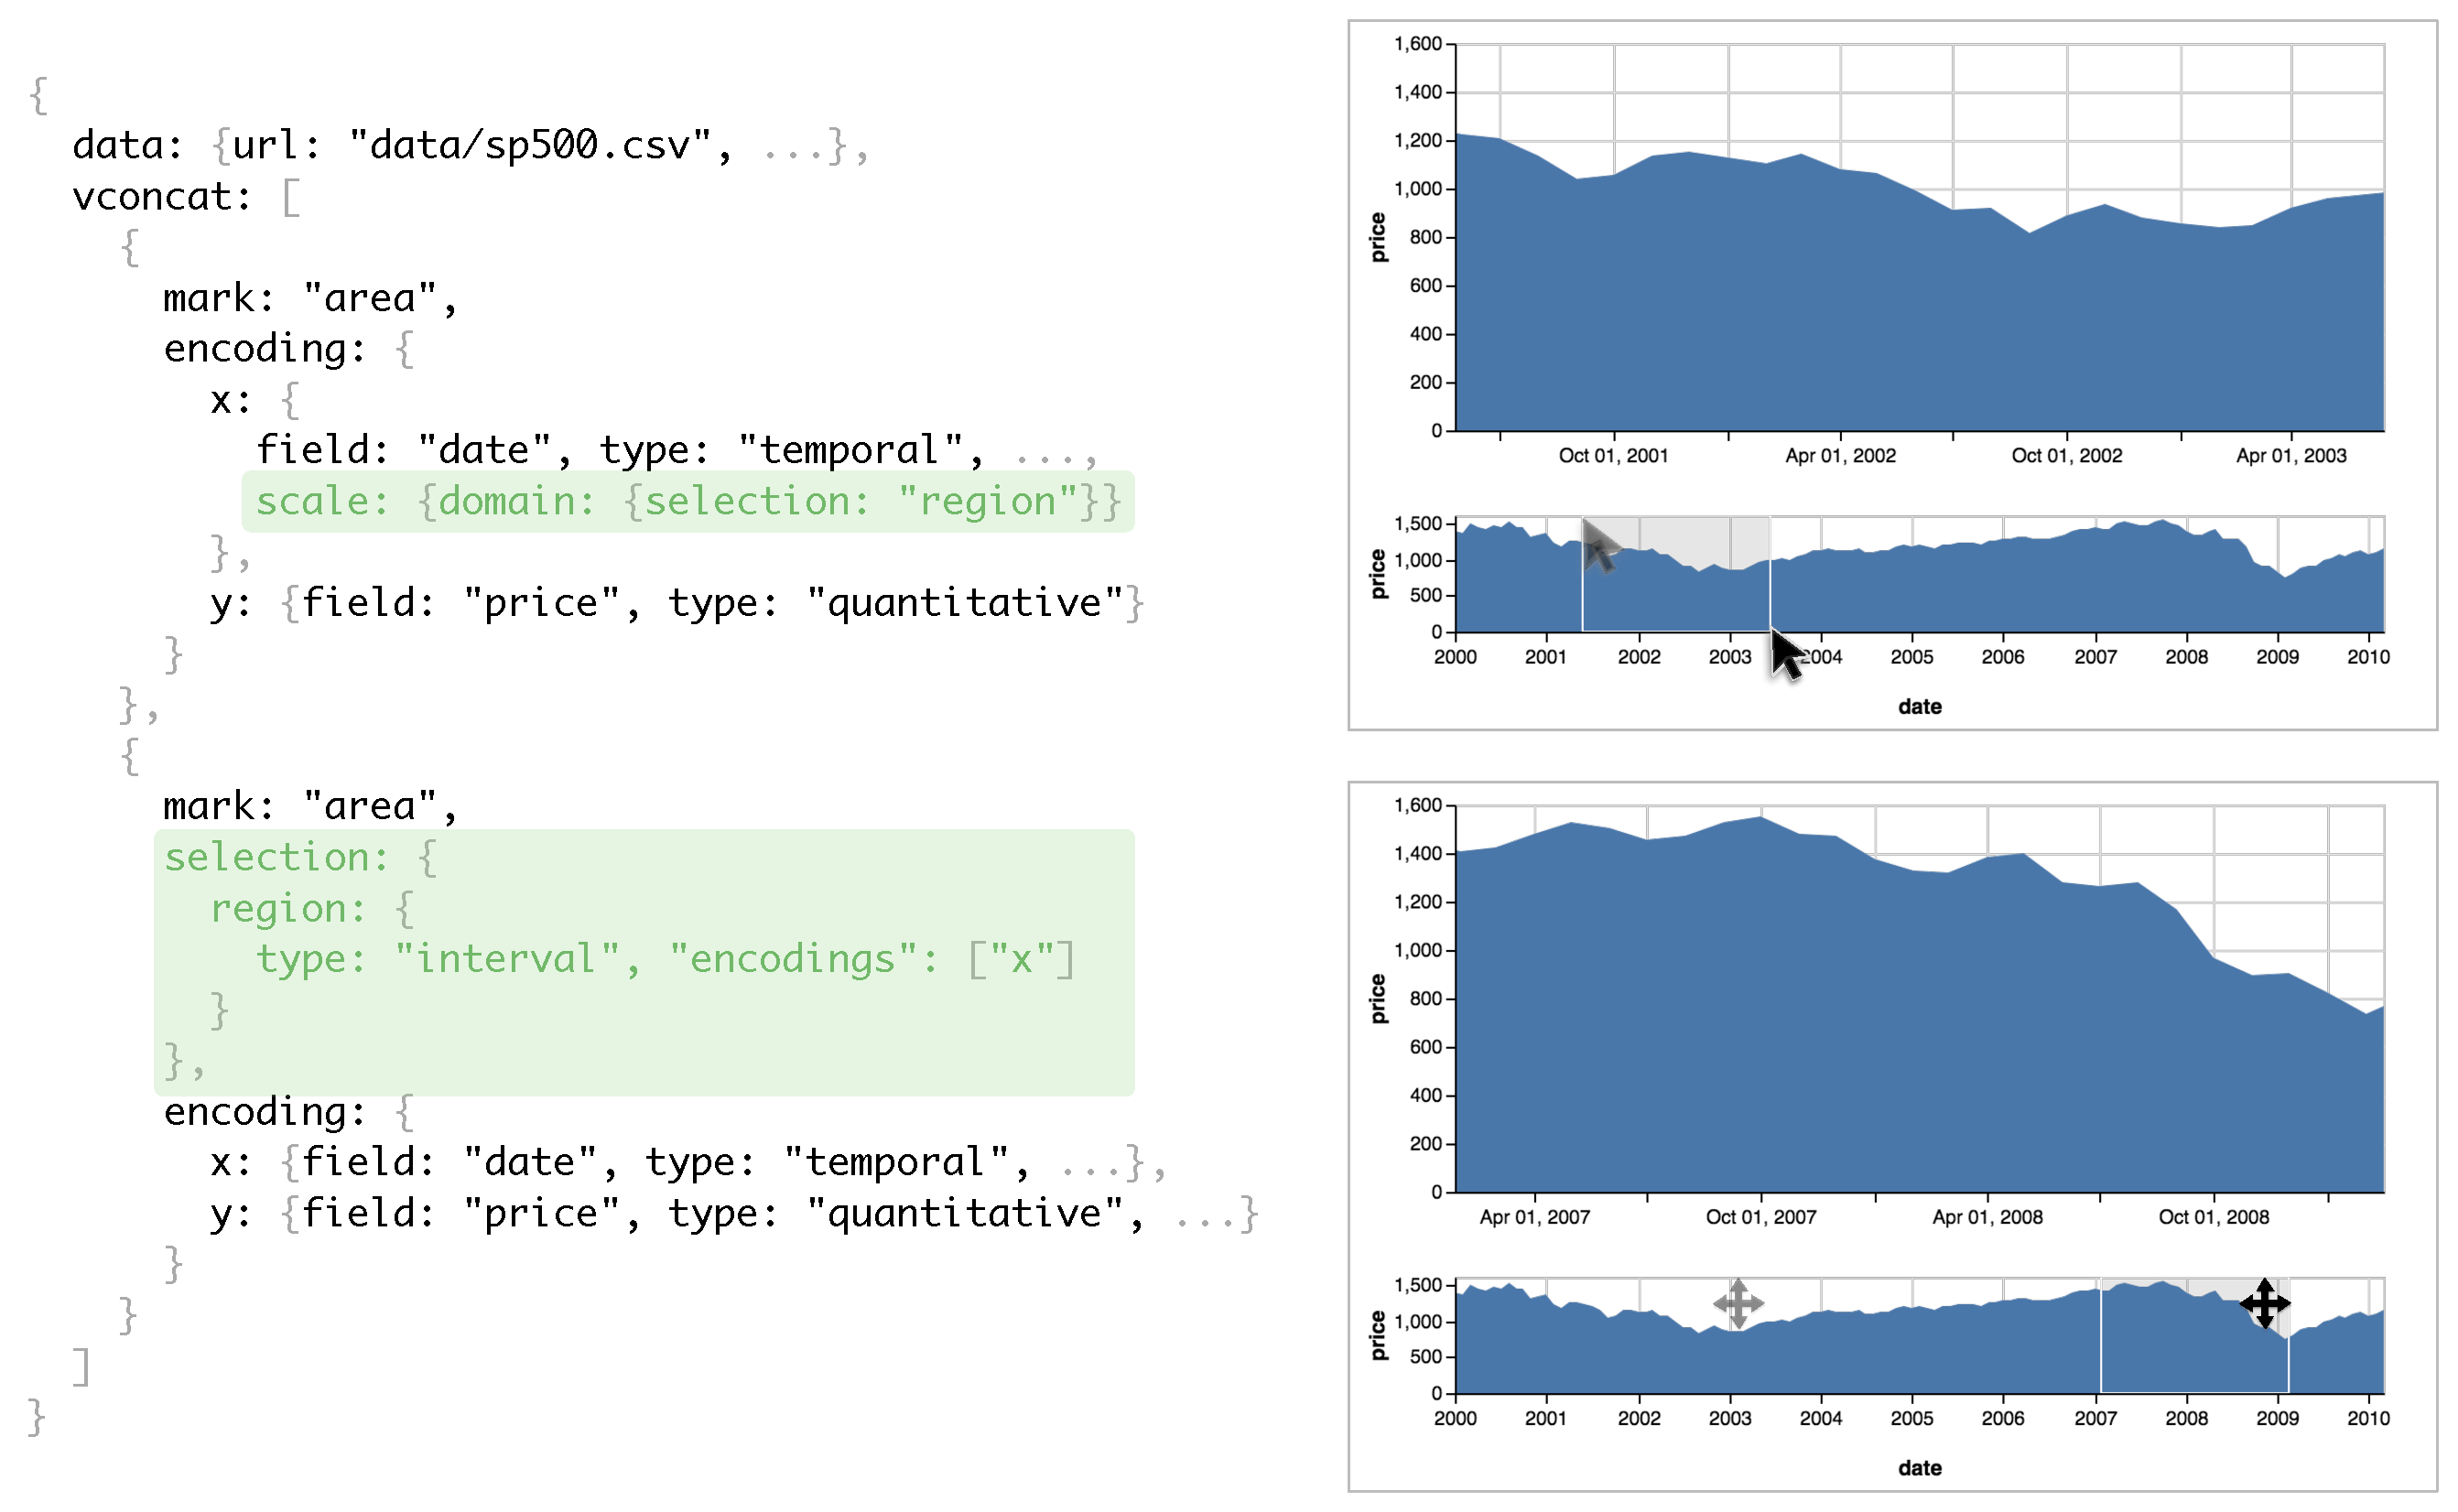
\includegraphics[width=\columnwidth]{overviewDetail}
  \caption{An overview\,+\,detail visualization concatenates two unit
  specifications, with a selection in the second one parameterizing the x-scale
  domain in the first.}
  \label{fig:vl:overviewDetail}
\end{figure}

\subsection{Reconfigure: Index Chart}

\Cref{fig:vl:indexChart} uses a single selection to interactively normalize
stock price time series data as the user moves their mouse across the chart. We
apply the \emph{nearest} transform to accelerate the selection using an
invisible Voronoi diagram. By projecting over the \texttt{date} field, the
selection represents both a single data value as well a set of values that share
the selected \texttt{date}. Thus, we can reference the single selection
directly, to position the red vertical rule, and also materialize it as part of
the \emph{lookup} data transform.

\begin{figure}[h!]
  \centering
  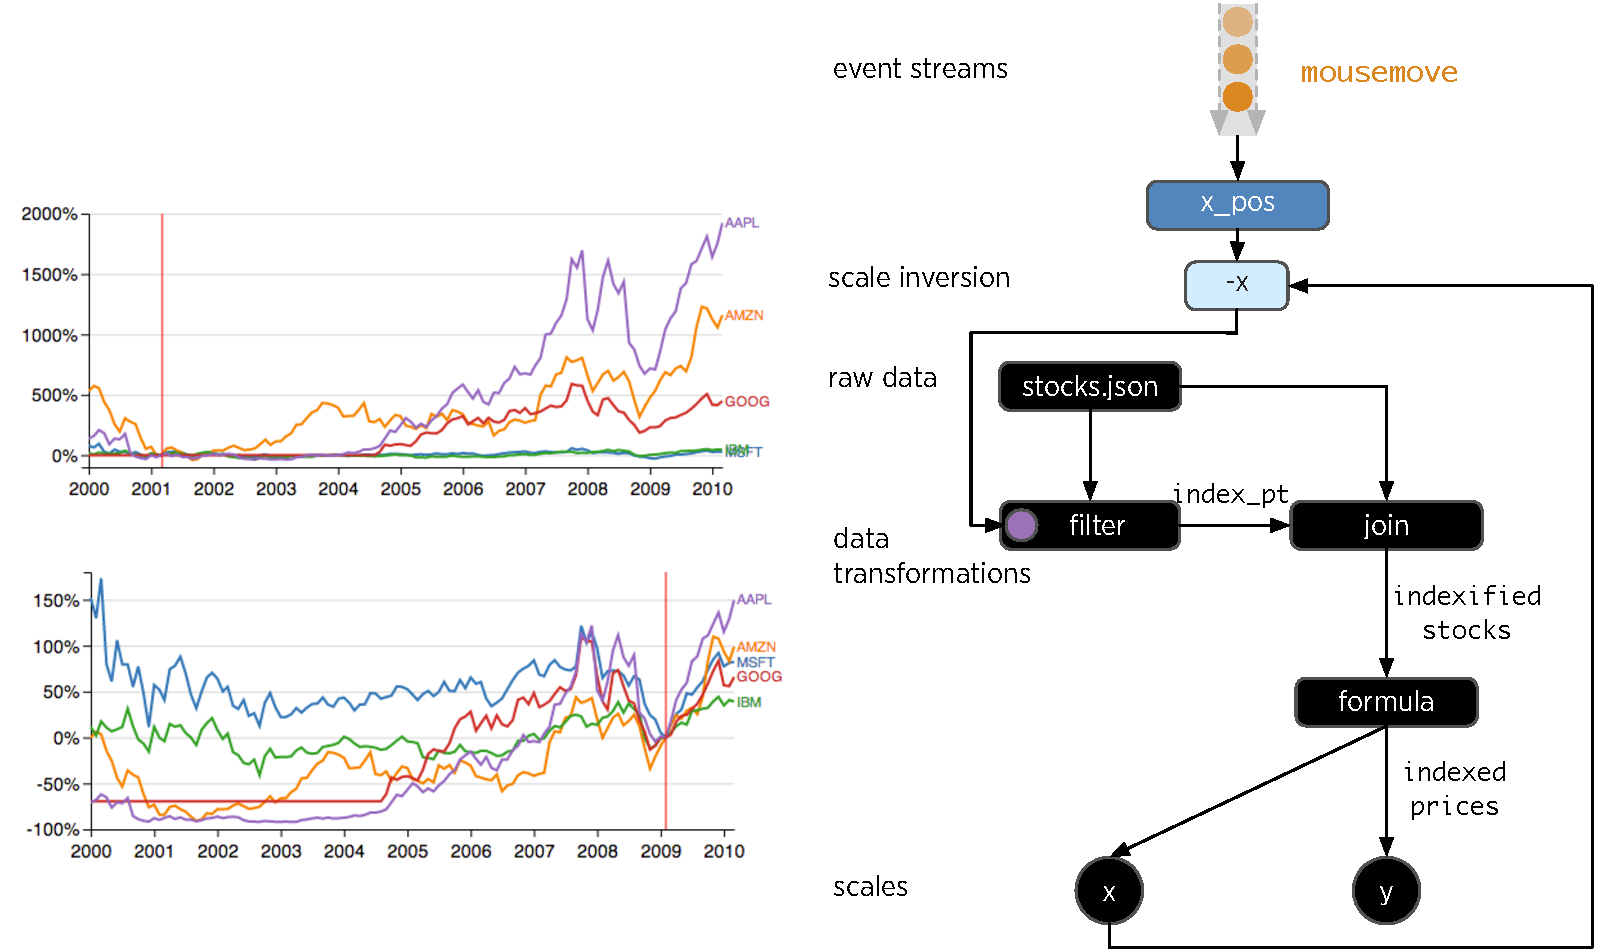
\includegraphics[width=\columnwidth]{indexChart}
  \caption{An index chart uses a single selection to renormalize data based
  on the index point nearest the mouse cursor.}
  \label{fig:vl:indexChart}
\end{figure}

\subsection{Filter: Cross Filtering}

As selections provide a predicate function, it is trivial to use them to filter
a dataset. \Cref{fig:vl:crossfilter}, for example, presents a concise
specification to enable filtering across three distinct binned histograms. It
uses a \emph{repeat} operator with a uni-dimensional interval selection over the
bins set to \emph{intersect others}. The \emph{filter} data transform applies
the selection against the backing datasets such that only data values that fall
within the selection are displayed. Thus, as the user brushes in one histogram,
the datasets that drive each of the other two are filtered, the data values are
re-aggregated, and the bars rise and fall. As with other interval selections,
the Vega-Lite compiler automatically instantiates the \emph{translate}
transform, allowing users to drag brushes around rather than having to reselect
them from scratch.

\begin{figure}[h!]
  \centering
  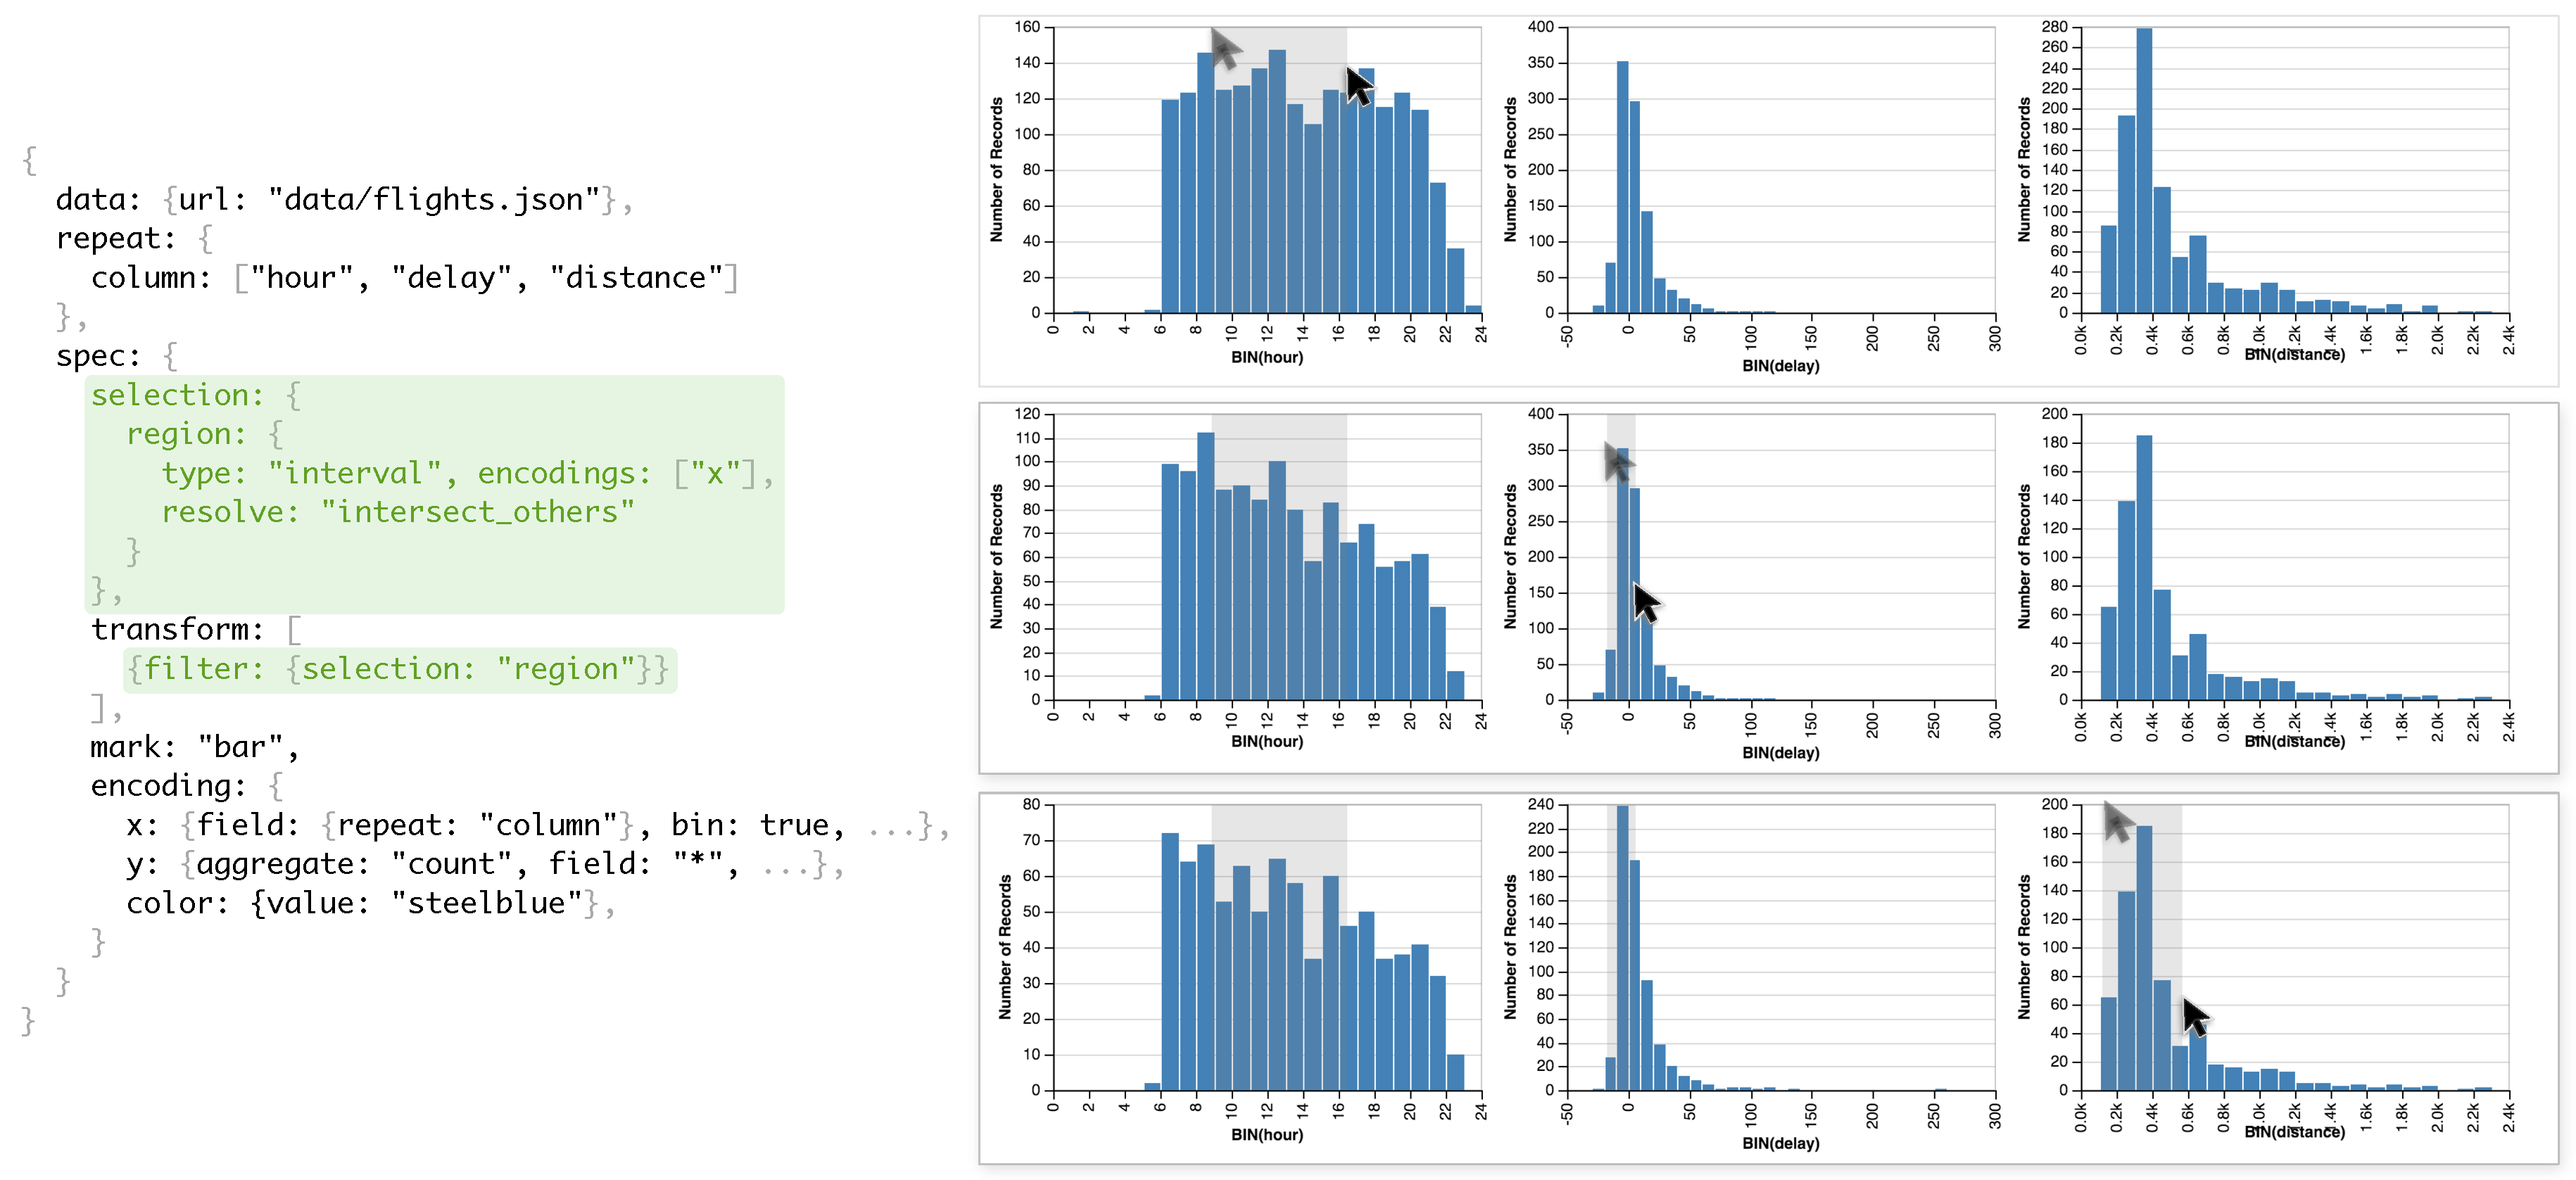
\includegraphics[width=\columnwidth]{crossfilter}
  \caption{An interval selection, resolved to \emph{intersect others}, drives a
  cross filtering interaction. Brushing in one histogram filters and
  reaggregates the data in the others, observable by the varying y-axis labels
  in the screenshots.}
  \label{fig:vl:crossfilter}
\end{figure}

The \emph{filter} data transform can also be used to materialize the selection
as an input dataset for secondary views. For instance, one drawback of
cross-filtering as in \cref{fig:vl:crossfilter} is that users only see the
selected values, and lose the context of the overall dataset. Instead of
applying the selection back onto the input dataset, we can instead materialize
it as an overlay (\cref{fig:vl:layeredCrossfilter}). Now, as the user brushes in
one histogram, bars highlight to visualize the proportion of the overall
distribution that falls within the brushed region(s). With this setup, it is
necessary to change the selection's resolution to simply \emph{intersect}, such
that bars in the brushed plot also highlight during the interaction.

\begin{figure}[h!]
  \centering
  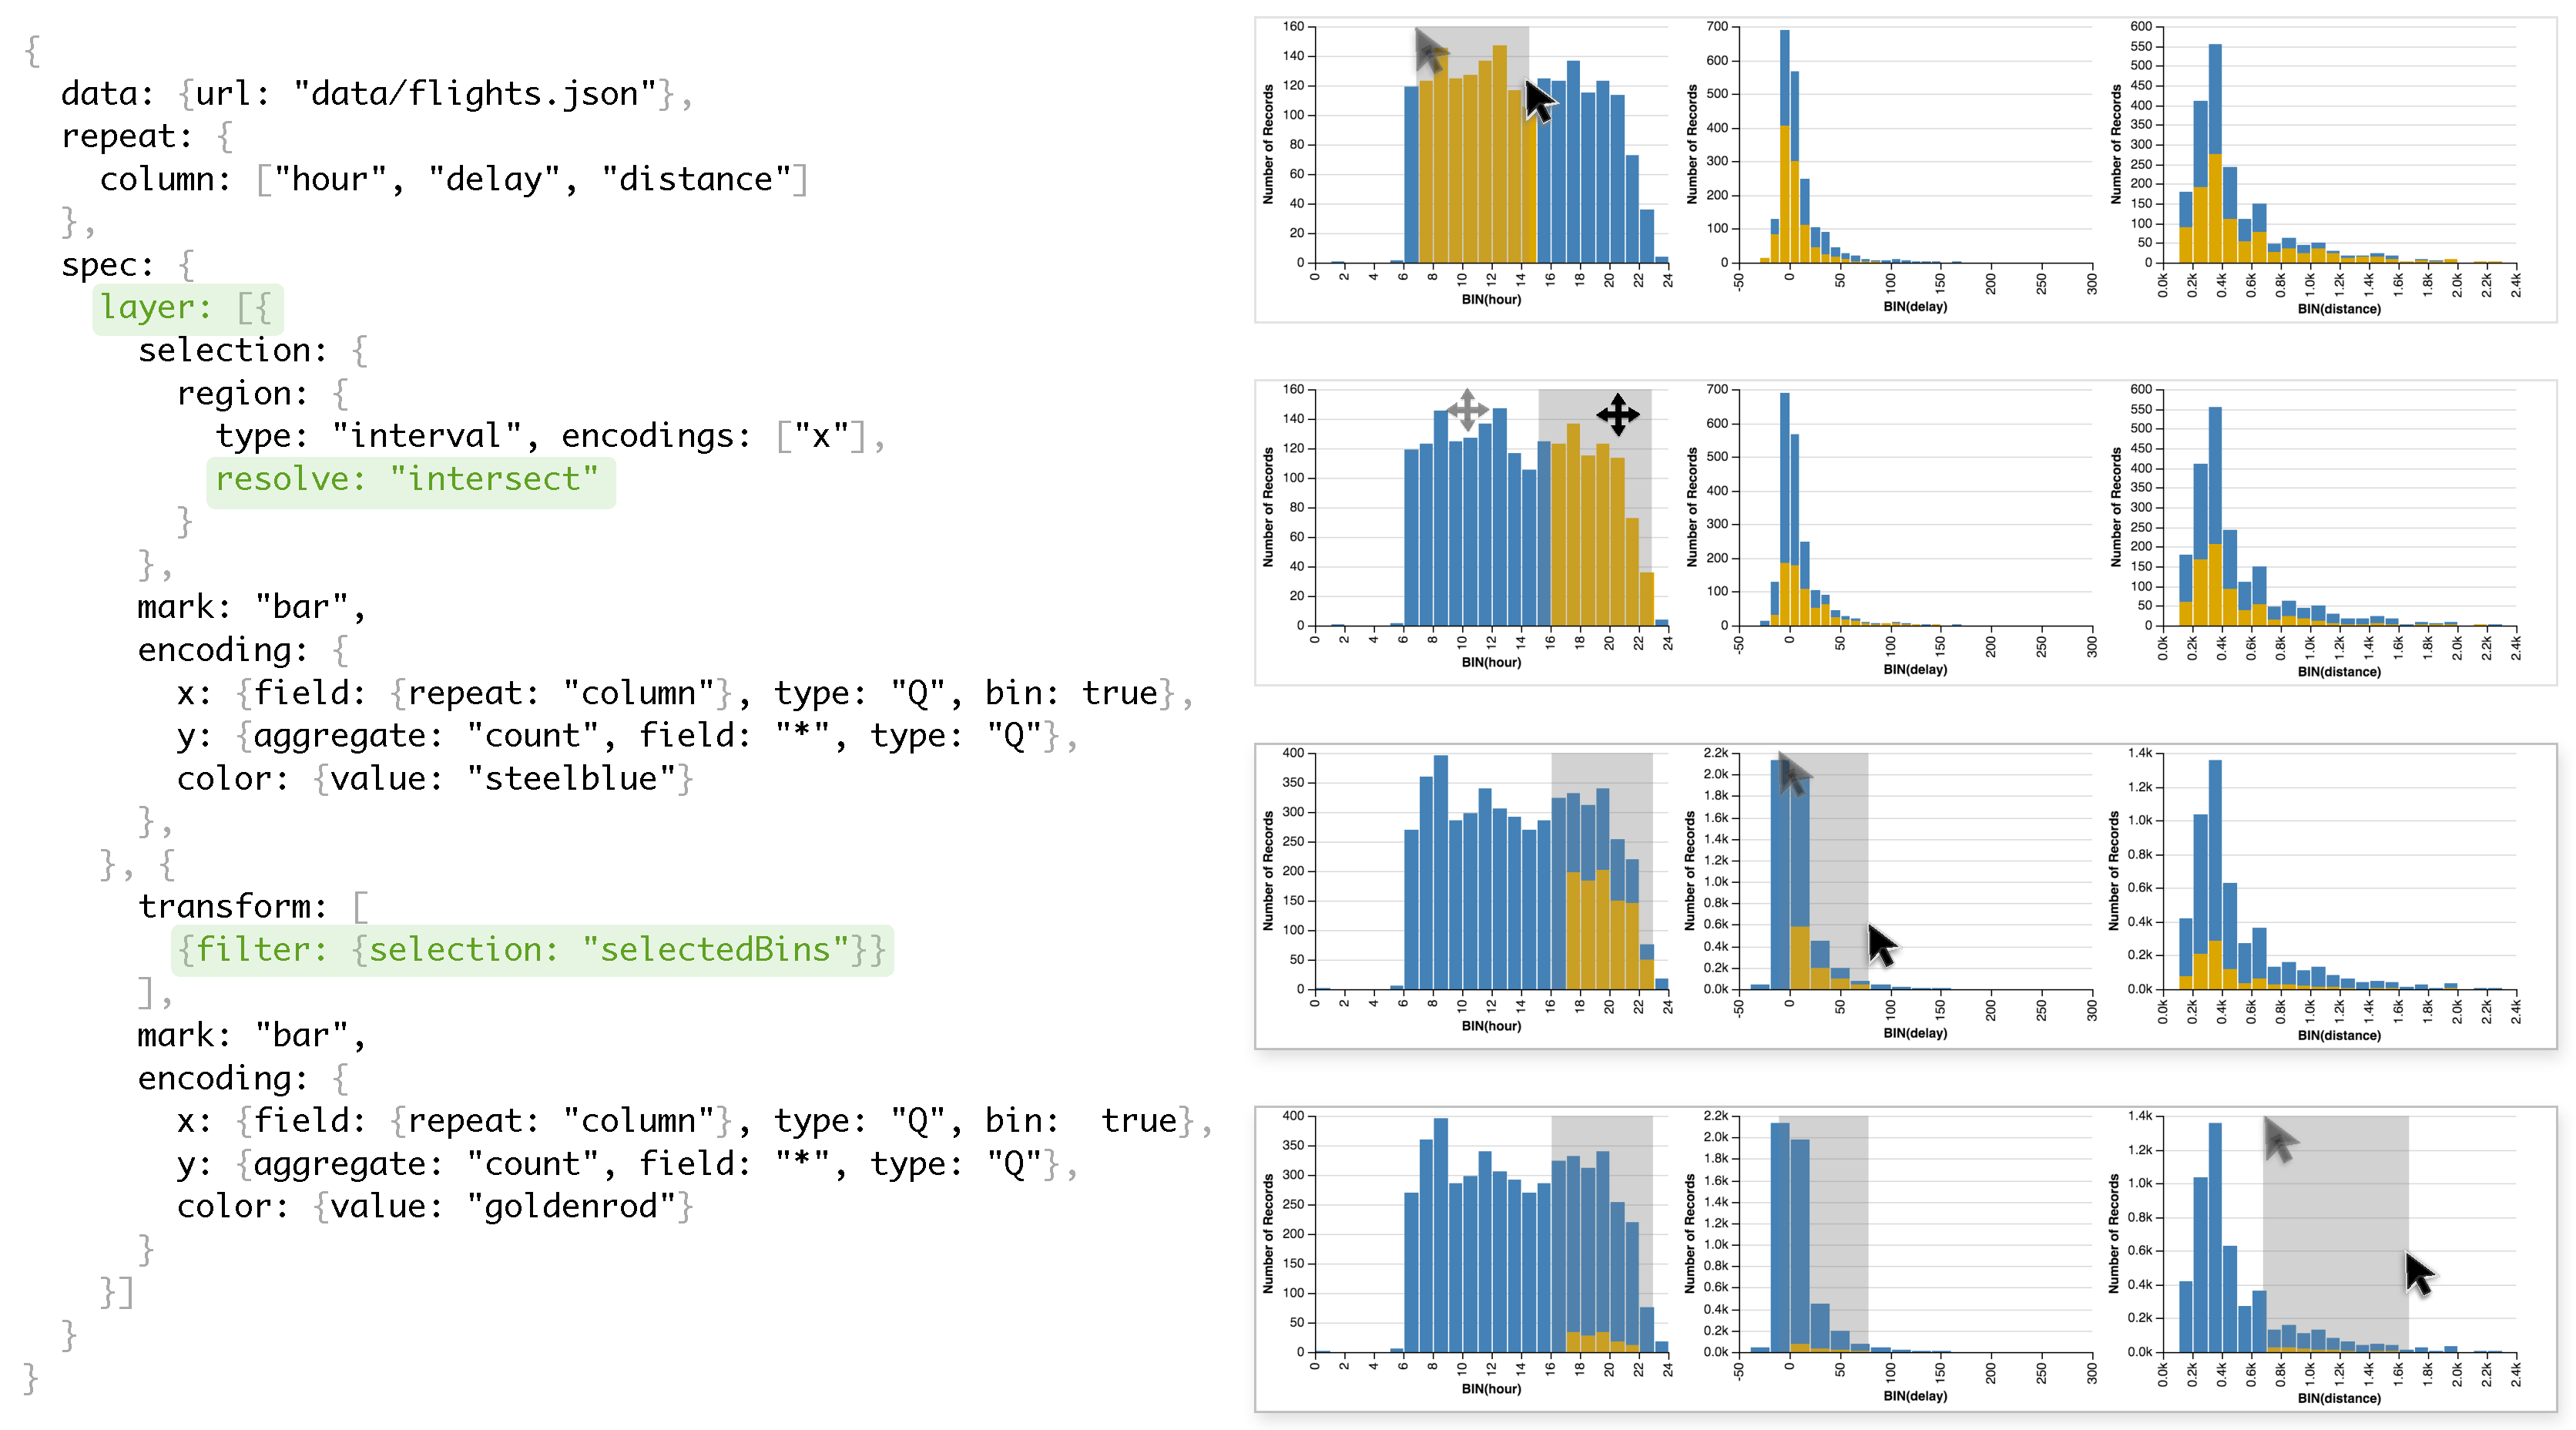
\includegraphics[width=\columnwidth]{layeredCrossfilter}
  \caption{A layered cross filtering interaction is constructed by resolving
  the interval selection to \emph{intersect}, and then materializing it to
  serve as the input data for a second layer. Highlights indicate changes to
  the specification from~\cref{fig:vl:crossfilter}.}
  \label{fig:vl:layeredCrossfilter}
\end{figure}

\subsection{Limitations}

The previous examples demonstrate that Vega-Lite specifications are more concise
than those of the lower-level Vega language, and yet are sufficiently expressive
to cover an interactive visualization taxonomy. Moreover, we have shown how
primitives can be systematically enumerated to facilitate exploration of
alternative designs. Nevertheless, we identify two classes of limitations that
currently exist.

First, there are limitations that are a result of how our formal model has been
reified in the current Vega-Lite implementation. In particular, components that
are determined at compile-time cannot be interactively manipulated. For example,
a selection cannot specify alternate fields to bin or aggregate over. Similarly,
more complex selection types (e.g., lasso selections) cannot be expressed as the
Vega-Lite system does not support arbitrary path marks. Such limitations can be
addressed with future versions of Vega-Lite, or alternate systems that
instantiate its grammar. For example, rather than a \emph{compiler},
interactions could parameterize the entirety of a specification within a
Vega-Lite \emph{interpreter}.

The second class of limitations are inherent to the model itself. As a
higher-level grammar, our model favors conciseness over expressivity. The
available primitives ensure that common methods can be rapidly specified, with
sufficient composition to enable more custom behaviors as well. However, highly
specialized techniques, such as querying time-series data via relaxed
selections~\cite{holz:relaxed}, cannot be expressed by default. Fortunately, our
formulation of selections, which decouple backing points from selected points
via a predicate function, provide a useful abstraction for extending our base
semantics with new, custom transforms. For example, the aforementioned technique
could be encapsulated in a \emph{relax} transform applicable to multi
selections.

While our selection abstraction supports \emph{interactive} linking of marks,
our view algebra does not yet provide means of \emph{visually} linking marks
across views (e.g., as in the Domino system~\cite{gratzl:domino}). Our view
algebra might be extended with support for connecting corresponding marks. For
example, points in repeated dot plots could be visually linked using line
segments to produce a parallel coordinates display.